\documentclass[journal]{IEEEtran}
\usepackage{amsmath,amsfonts}
\usepackage{algorithmic}
\usepackage{algorithm}
\usepackage{amssymb}
\usepackage{array}
\usepackage[caption=false,font=normalsize,labelfont=sf,textfont=sf]{subfig}
\usepackage{textcomp}
\usepackage{stfloats}
\usepackage{url}
\usepackage{verbatim}
\usepackage{graphicx}
\usepackage{cite}
\usepackage{xcolor}
\hyphenation{op-tical net-works semi-conduc-tor IEEE-Xplore}
\usepackage{hyperref}
\hypersetup{
  colorlinks=true,   % Enable colored links
  linkcolor=blue,    % Set internal links to blue
  citecolor=blue,    % Set citation links to blue
  urlcolor=blue      % Set URL links to blue
}
\usepackage{booktabs} % for \hline
\renewcommand{\algorithmicrequire}{\textbf{Input:}}
\renewcommand{\algorithmicensure}{\textbf{Output:}}
\usepackage{threeparttable}
\usepackage{amsthm}
\newtheorem{definition}{Definition}
\newtheorem{proposition}{Proposition}
\usepackage{listings}
\usepackage{tikz}
\usetikzlibrary{shapes,arrows,positioning,calc,shadows,decorations.pathreplacing,fit}
\usepackage{multirow}

%=============Suggested================
% - the fig:optimization_architecture can zoom out the figure font size.
%=============Suggested================

\begin{document}

\title{Thread-Adaptive: Optimized Parallel Architectures of SLH-DSA on GPUs}

\author{Jiahao Xiang and Lang Li.

  \thanks{This work is supported by the Hunan Provincial Natural Science Foundation of China (2022JJ30103), Postgraduate Scientific Research Innovation Project of Hunan Province (CX20240977), “the 14th Five-Year Plan” Key Disciplines and Application-oriented Special Disciplines of Hunan Province (Xiangjiaotong [2022] 351), the Science and Technology Innovation Program of Hunan Province (2016TP1020).}

  \thanks{Jiahao Xiang and Lang Li are affiliated with the Hunan Provincial Key Laboratory of Intelligent Information Processing and Application, as well as the Hunan Engineering Research Center of Cyberspace Security Technology and Applications, both located at Hengyang Normal University, Hengyang 421002, China. They are also faculty members of the College of Computer Science and Technology at Hengyang Normal University. (e-mail: jiahaoxiang2000@gmail.com; lilang911@126.com)}% <-this % stops a space
}
% \thanks{Manuscript received April 19, 2021; revised August 16, 2021.}}
% \thanks{Manuscript received }}

% The paper headers
\markboth{Journal of \LaTeX\ Class Files,~Vol.~14, No.~8, August~2021}%
{Shell \MakeLowercase{\textit{et al.}}: A Sample Article Using IEEEtran.cls for IEEE Journals}

\IEEEpubid{}
% Remember, if you use this you must call \IEEEpubidadjcol in the second
% column for its text to clear the IEEEpubid mark.

\maketitle

\begin{abstract}
  The imminent threat posed by quantum computing necessitates an urgent transition to Post-Quantum Cryptography (PQC) to safeguard sensitive data against future cryptanalytic attacks.
  The stateless hash-based digital signature algorithm (SLH-DSA) FIPS 205, while quantum-resistant, presents significant computational challenges for practical deployment.
  This research presents a GPU-accelerated implementation of SLH-DSA that employs a thread-adaptive parallelization methodology to maximize throughput.
  In contrast to conventional approaches utilizing fixed maximum thread allocation, the proposed implementation dynamically optimizes parallelism levels for individual cryptographic kernel functions, thereby establishing an equilibrium between thread utilization and execution efficiency.
  Furthermore, granular decomposition of signature components is implemented to enhance thread-level execution performance.
  Performance evaluation conducted on an NVIDIA RTX 4090 GPU demonstrates that the implementation attains a throughput of 62,239 signatures per second for the SPHINCS$^+$-128f parameter set, representing a significant performance improvement over existing methodologies.
  The empirical results establish GPUs as viable platforms for SLH-DSA acceleration in high-throughput environments, thus facilitating the practical transition to post-quantum cryptographic standards.

\end{abstract}

\begin{IEEEkeywords}
  FIPS 205, GPU, SPHINCS\textsuperscript{+}, Signature algorithm.
\end{IEEEkeywords}

\section{Introduction}
\label{sec:intro}

\IEEEPARstart{Q}{uantum} computers pose a significant threat to current cryptographic systems through their ability to efficiently solve mathematical problems that underpin modern security protocols. This threat materializes in the anticipated ``Q-Day", when quantum computers attain sufficient computational power to compromise public encryption systems safeguarding digital communications, authentication mechanisms, and key exchange protocols. Widely deployed public-key cryptosystems such as RSA and ECC are particularly vulnerable to Shor's algorithm, which can efficiently factor large integers and compute discrete logarithms problems considered computationally infeasible using classical computing approaches \cite{Yang2023}.
In response to these vulnerabilities, the National Institute of Standards and Technology (NIST) initiated the Post-Quantum Cryptography (PQC) standardization process to develop cryptographic schemes resistant to quantum computing capabilities. The imminent threat of encrypted data being harvested now for future decryption once quantum computing matures makes the transition to post-quantum cryptography increasingly urgent for protecting sensitive information and maintaining long-term data security.

SPHINCS\textsuperscript{+}, a prominent stateless hash-based signature scheme and NIST standardization finalist \cite{Yesina}, provides robust quantum-attack resistance through secure cryptographic hash functions \cite{Bernstein2019}. This scheme subsequently formed the foundation for the Stateless Hash-based Digital Signature Algorithm (SLH-DSA), now standardized as FIPS 205 \cite{FIPS205}. The computational intensity of these hash-based signatures has necessitated research into efficient implementations across various hardware platforms, including CPUs, FPGAs, and GPUs \cite{Joseph2022}, to facilitate organizational transitions to post-quantum cryptographic solutions.

\subsection{Related Work}

GPU acceleration for SPHINCS\textsuperscript{+} has evolved substantially in recent years. Lee and Hwang~\cite{Lee2022} established the fundamental parallel implementation techniques for hash-based signatures, demonstrating the viability of GPU acceleration for post-quantum cryptography. Building on this foundation, Kim et al.~\cite{Kim2024} developed parallel methods for critical SPHINCS\textsuperscript{+} components—specifically FORS, WOTS\textsuperscript{+}, and Merkle tree computations. Their implementation on the NVIDIA RTX 3090 achieved significant throughput improvements, despite efficiency constraints from multiple kernel invocations.

Subsequently, Wang et al.~\cite{Wang2025} introduced CUSPX, a sophisticated three-level parallelism framework integrating algorithmic, data, and hybrid parallelization approaches. Their implementation featured optimized parallel Merkle tree construction algorithms and strategic load-balancing techniques, resulting in substantial performance enhancements.

\subsection{Motivation}

Existing GPU implementations of SLH-DSA reveals two fundamental efficiency constraints.
First, conventional approaches apply uniform thread allocation across all cryptographic operations, neglecting the distinct computational characteristics of individual functions. This static resource allocation creates significant imbalances certain operations suffer from excessive synchronization overhead while others underutilize available computational resources.

Second, the hierarchical structure of SLH-DSA, comprising multiple hash operations distributed across FORS, WOTS\textsuperscript{+}, and Merkle tree components, permits decomposition into smaller computational units. However, current implementations emphasize maximizing thread count rather than optimizing computational efficiency, resulting in suboptimal per-thread performance despite high hardware utilization rates.
These limitations necessitate an adaptive parallelization approach that dynamically determines optimal thread configurations for specific cryptographic functions while enabling fine-grained decomposition of signature components.

\subsection{Contributions}

This paper presents a thread-adaptive GPU-based implementation of SLH-DSA with the following key contributions:

\begin{enumerate}
  \item A dynamic thread allocation methodology that optimizes thread configurations for individual cryptographic functions based on their computational characteristics, effectively balancing parallelism with execution efficiency to minimize synchronization overhead while maximizing throughput.

  \item A sophisticated function-level parallelization approach that strategically decomposes cryptographic operations into independent computational tasks, significantly reducing latency and enhancing the performance of core SLH-DSA primitives.

  \item Performance evaluation on NVIDIA GPU architecture demonstrating a throughput of 62,239 SLH-DSA signatures per second (for SPHINCS$^+$-128f), representing substantial improvement over state-of-the-art implementations.
    The complete implementation is available as an open-source repository at \url{https://github.com/jiahaoxiang2000/sphincs-plus}.
\end{enumerate}

The paper is structured as follows: Section~\ref{sec:preliminaries} presents the fundamental concepts of the SLH-DSA signature scheme; Section~\ref{sec:implementation} describes the architectural design and implementation details; Section~\ref{sec:evaluation} analyzes performance results and comparative metrics; and Section~\ref{sec:conclusion} summarizes findings and discusses future research directions.

\section{Preliminaries}\label{sec:preliminaries}

\subsection{SLH-DSA Overview}

SLH-DSA represents a stateless hash-based signature scheme that provides post-quantum security through hierarchical certification architecture. The signature generation mechanism comprises three fundamental components:

\begin{itemize}
  \item \textbf{WOTS\textsuperscript{+} (Winternitz One-Time Signature)}: A one-time scheme facilitating authentication paths and supporting Merkle tree construction
  \item \textbf{FORS (Forest Of Random Subsets)}: A few-time signature scheme utilizing $k$ components, each containing $t$ elements selected from pseudorandom subsets
  \item \textbf{Hypertree}: A multi-layer structure with height $h$ divided into $d$ layers, each containing Merkle trees of height $h/d$ for WOTS\textsuperscript{+} public key authentication
\end{itemize}

\begin{figure}[t]
  \centering
  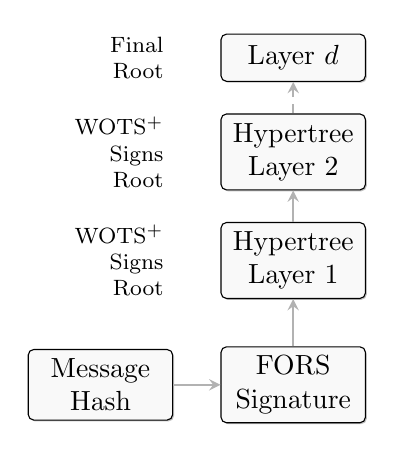
\begin{tikzpicture}[
      block/.style={
        rectangle,
        draw,
        fill=white,
        text width=1.6cm,
        align=center,
        minimum height=0.6cm,
        rounded corners=2pt,
        fill=gray!5,
        drop shadow={shadow xshift=0.5pt, shadow yshift=-0.5pt}
      },
      arrow/.style={->,>=stealth,thick,draw=gray!60},
      level/.style={sibling distance=35mm,level distance=0.7cm}
    ]
    % Message and Components
    \node[block] (fors) at (0,0) {FORS\\Signature};
    \node[block,left=0.6cm of fors] (hash) {Message\\Hash};

    % Hypertree Layers
    \node[block,above=0.6cm of fors] (ht1) {Hypertree\\Layer 1};
    \node[block,above=0.4cm of ht1] (ht2) {Hypertree\\Layer 2};
    \node[block,above=0.4cm of ht2] (htd) {Layer $d$};

    \draw[arrow] (hash) to (fors);
    \draw[arrow] (fors) to (ht1);
    \draw[arrow] (ht1) to (ht2);
    \draw[arrow] ($(htd)+(0,-0.5)$) -- (htd);
    \draw[dashed,thick,gray!60] ($(ht2)+(0,0.5)$) -- ($(htd)+(0,-0.3)$);

    \node[left=0.6cm of ht1,text width=1.4cm,font=\footnotesize,align=right] {WOTS\textsuperscript{+} Signs Root};
    \node[left=0.6cm of ht2,text width=1.4cm,font=\footnotesize,align=right] {WOTS\textsuperscript{+} Signs Root};
    \node[left=0.6cm of htd,text width=1.4cm,font=\footnotesize,align=right] {Final Root};
  \end{tikzpicture}
  \caption{SLH-DSA signature generation flow. A message hash undergoes FORS signing to produce $k$ authentication paths, subsequently authenticated by a $d$-layer hypertree. Each layer employs WOTS\textsuperscript{+} to sign the previous layer's root, culminating in a final root signature.}
  \label{fig:sphincs-process}
\end{figure}

The SLH-DSA signature generation process, illustrated in Fig.~\ref{fig:sphincs-process}, implements a hierarchical authentication structure. Initially, a message digest is generated through hashing, followed by FORS few-time scheme signing, which produces $k$ authentication paths comprising $t$ elements each. The resulting FORS public key undergoes authentication via a $d$-layer hypertree, where each layer applies WOTS\textsuperscript{+} to sign the lower layer's root. This signature chain terminates at the final root node, enabling efficient verification while maintaining robust hash-based security.

SLH-DSA offers ``simple" and ``robust" operational modes to optimize speed-security trade-offs. Various parameter sets accommodate different requirements regarding signature size, security level, and computational efficiency. The scheme derives all security properties from underlying hash functions, rendering it resistant to quantum computational attacks.

\subsection{GPU Computing Model}

Graphics Processing Units (GPUs) incorporate numerous cores organized within Streaming Multiprocessors (SMs). This parallel architecture implements Single Instruction, Multiple Thread (SIMT) execution, organizing threads into warps that collectively form blocks. These blocks are distributed across available SMs, enabling thousands of concurrent threads to execute similar instructions simultaneously.

The CUDA framework enhances computational throughput through memory optimization strategies including coalesced memory accesses, shared memory utilization, and constant memory buffering. These techniques facilitate extensive parallelization of SLH-DSA computations, yielding performance improvements through the combined application of thread-level, data-level, and algorithmic parallelism.

\section{Optimized Implementation of SLH-DSA}\label{sec:implementation}

This section presents a novel optimization framework for SLH-DSA that employs a dual-component architecture, as illustrated in Fig.~\ref{fig:optimization_architecture}. The framework integrates Adaptive Thread Allocation (ATA) with Function-Level Parallelism (FLP) to maximize computational efficiency while preserving cryptographic integrity.

\begin{figure*}[htbp]
  \centering
  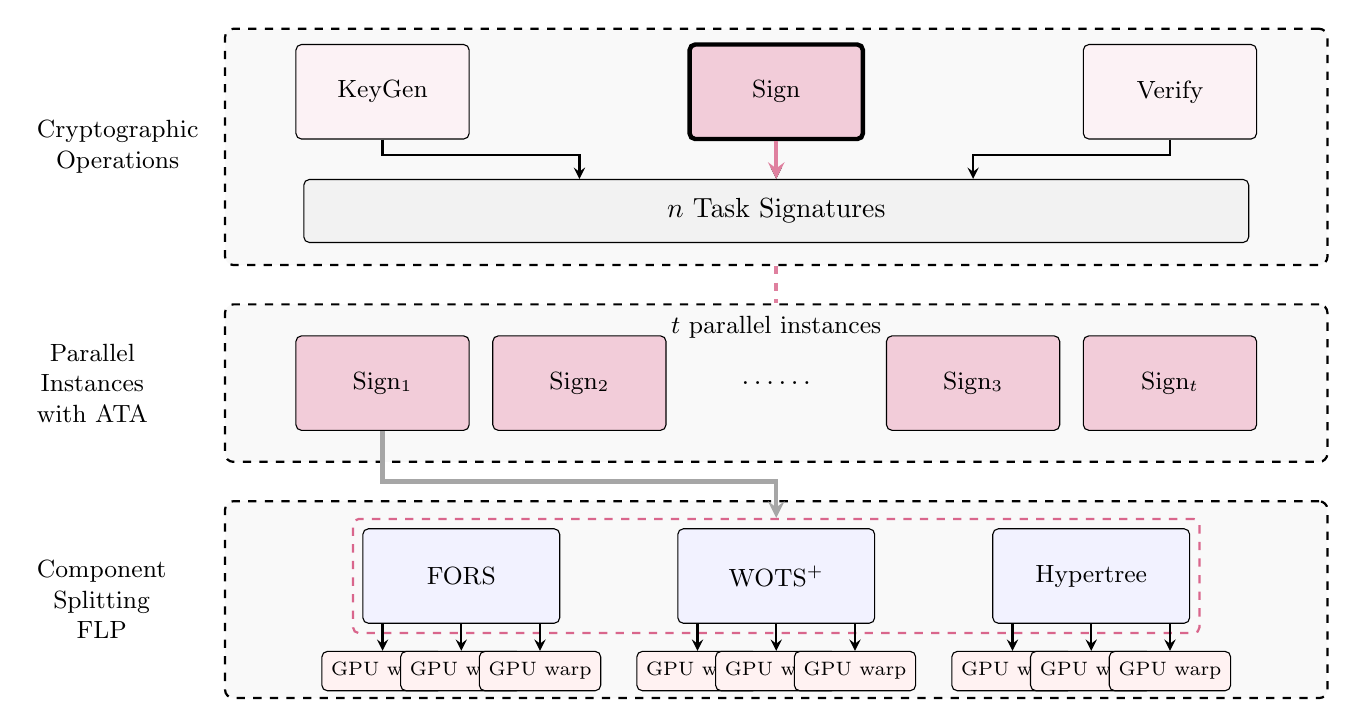
\begin{tikzpicture}[
      % Define styles with better semantic meaning
      layer/.style={draw, rounded corners=3pt, dashed, thick, fill=gray!5, minimum width=14cm, minimum height=2.5cm},
      task/.style={draw, rounded corners=2pt, minimum width=2.2cm, minimum height=1.2cm, align=center, font=\small, fill=purple!5},
      selected/.style={task, fill=purple!20, ultra thick},
      component/.style={draw, rounded corners=2pt, minimum width=2.5cm, minimum height=1.2cm, align=center, font=\small, fill=blue!5},
      gpu/.style={draw, rounded corners=2pt, minimum width=1.1cm, minimum height=0.5cm, font=\scriptsize, align=center, fill=red!5},
      arrow/.style={->, >=stealth, thick},
      manyarrows/.style={->, >=stealth, thick, draw=gray!70},
      highlightarrow/.style={->, >=stealth, thick, draw=purple!60, dashed},
      highlightbox/.style={draw, rounded corners=2pt, dashed, thick, draw=purple!60, fit=#1}
    ]

    % Layer boxes with vertical stacking
    \node[layer, anchor=north, minimum width=14cm, minimum height=3cm] (layer1) at (0,4.5) {};
    \node[layer, anchor=north, minimum width=14cm, minimum height=2cm] (layer2) at (0,1.0) {};
    \node[layer, anchor=north] (layer3) at (0,-1.5) {};

    % Layer labels - positioned relative to each layer
    \node[align=center, font=\small, anchor=west] at ($(layer1.west) + (-2.5,0)$) {Cryptographic\\Operations};
    \node[align=center, font=\small, anchor=west] at ($(layer2.west) + (-2.5,0)$) {Parallel\\Instances\\with ATA};
    \node[align=center, font=\small, anchor=west] at ($(layer3.west) + (-2.5,0)$) {Component\\Splitting\\FLP};

    % Signature tasks with horizontal positioning in top layer
    \node[task] (keygen) at ($(layer1.center) + (-5,0.7)$) {KeyGen};
    \node[selected] (sign) at ($(layer1.center) + (0,0.7)$) {Sign};
    \node[task] (verify) at ($(layer1.center) + (5,0.7)$) {Verify};

    % Task queue - positioned relative to the layer
    \node[draw, rounded corners=2pt, fill=gray!10, minimum width=12cm, minimum height=0.8cm]
    (queue) at ($(layer1.south) + (0,0.7)$) {$n$ Task Signatures};

    % Connect tasks to queue using relative positioning
    \foreach \op/\pos in {keygen/-5, sign/0, verify/5} {
      \draw[arrow] (\op) -- ++(0,-0.8) -| ($(queue.north) + (\pos/2,0)$);
    }

    % Highlight the selected task path
    \draw[arrow, ultra thick, draw=purple!50] (sign) -- ++(0,-0.8) -| (queue);

    % Changed to dashed line for middle arrow
    \draw[ultra thick, draw=purple!50, dashed] (layer1.south) -- ($(layer2.north) + (0,0)$);

    % Label for instances - positioned relative to the connection
    \node[font=\small] at ($(layer2.north) + (0,-0.3)$) {$t$ parallel instances};

    % Multiple instances of sign task - positioned relative to middle layer
    \foreach \i/\pos in {1/-5,2/-2.5,3/2.5} {
      \node[task, fill=purple!20] (sign\i) at ($(layer2.center) + (\pos,0)$) {Sign$_{\i}$};
    }
    \node[task, fill=purple!20] (signt) at ($(layer2.center) + (5,0)$) {Sign$_{t}$};

    \node at ($(layer2.center) + (0,0)$) {$\ldots \ldots$};

    % Component splitting - positioned relative to bottom layer
    \node[component] (fors) at ($(layer3.center) + (-4,0.3)$) {FORS};
    \node[component] (wots) at ($(layer3.center) + (0,0.3)$) {WOTS\textsuperscript{+}};
    \node[component] (hypertree) at ($(layer3.center) + (4,0.3)$) {Hypertree};

    % Highlight Sign1 expanding to FLP layer
    \node[highlightbox={(fors) (wots) (hypertree)}] (flpbox) {};
    \draw[manyarrows, ultra thick] (sign1.south) -- ($(layer2.south)!0.5!(layer3.north) + (-5,0)$) --
    ($(layer2.south)!0.5!(layer3.north) + (0,0)$) -- (flpbox.north);

    % GPU Blocks - positioned relative to components
    \foreach \comp/\name/\pos in {fors/FORS/-4, wots/WOTS/0, hypertree/Hypertree/4} {
      \foreach \shift in {-1, 0, 1} {
        \node[gpu] (gpu\name\shift) at ($(\comp.south) + (\shift,-0.6)$) {GPU warp};
        \draw[arrow] ($(\comp.south) + (\shift,-0.0)$) -- (gpu\name\shift);
      }
    }

  \end{tikzpicture}
  \caption{Thread-adaptive parallelization architecture for SLH-DSA. The architecture comprises three hierarchical layers: the top layer represents cryptographic operations (with Sign highlighted); the middle layer implements Adaptive Thread Allocation (ATA) with dynamically optimized thread configurations distributed across $t$ parallel instances; the bottom layer employs Function-Level Parallelism (FLP) by decomposing operations into algorithmic components (FORS, WOTS\textsuperscript{+}, and Hypertree). Each component distributes computation across multiple GPU warps, with each warp containing 32 threads as the fundamental execution unit.}
  \label{fig:optimization_architecture}
\end{figure*}

\subsection{Adaptive Thread Allocation}

Conventional GPU implementations of cryptographic algorithms typically apply maximum thread allocation universally, neglecting the distinct computational profiles of individual operations within SLH-DSA. Our research introduces a thread-adaptive methodology that precisely calibrates parallelization based on function-specific characteristics to achieve optimal performance.

\subsubsection{Performance Modeling}

The execution time for each cryptographic function $g_i$ in SLH-DSA is characterized by:

\begin{equation}
  \label{eq:execution_time_model}
  T(g_i, t) = \alpha_i + \frac{\beta_i}{t} + \gamma_i \cdot t,
\end{equation}
This model captures three essential components: $\alpha_i$ represents invariant computational overhead independent of thread count, $\frac{\beta_i}{t}$ reflects the parallelizable workload component that scales inversely with thread count, and $\gamma_i \cdot t$ quantifies thread management overhead that increases linearly with thread allocation. The formulation encapsulates the fundamental parallelization tradeoff between computational acceleration and synchronization costs.

\subsubsection{Optimal Thread Determination}

By minimizing $T(g_i, t)$ with respect to $t$, the optimal thread allocation $t_i^*$ for each function is derived as:

\begin{equation}
  \label{eq:optimal_thread_count}
  t_i^* = \sqrt{\frac{\beta_i}{\gamma_i}},
\end{equation}
The parameters $\alpha_i$, $\beta_i$, and $\gamma_i$ were determined through systematic profiling of each cryptographic operation across multiple thread configurations, establishing an empirical foundation for optimization decisions.

\subsubsection{Dynamic Implementation}

The thread allocation optimization follows the methodology outlined in Algorithm~\ref{alg:adaptive_thread_allocation}.

\begin{algorithm}
  \caption{Adaptive Thread Allocation (ATA)}
  \label{alg:adaptive_thread_allocation}
  \begin{algorithmic}[1]
    \REQUIRE Set of cryptographic functions $G = \{g_1, g_2, \ldots, g_m\}$
    \ENSURE Optimized thread configuration for each function

    \FOR{each function $g_i \in G$}
    \STATE Profile $g_i $ with varying thread counts $t \in \{2^j | j \in [5, 10]\}$
    \STATE Fit performance data to model $T(g_i, t) = \alpha_i + \frac{\beta_i}{t} + \gamma_i \cdot t$
    \STATE Calculate $t_i^* = \sqrt{\frac{\beta_i}{\gamma_i}}$
    \STATE Round $t_i^*$ to nearest power of 2 for GPU scheduler compatibility
    \ENDFOR

    \STATE Store thread configuration in constant memory lookup table
    \RETURN Thread configuration table
  \end{algorithmic}
\end{algorithm}

This architecture dynamically balances parallelism against synchronization overhead, yielding precise resource allocation tailored to each cryptographic operation. The thread configuration resides in GPU constant memory for low-latency access during execution, ensuring computational efficiency without introducing additional runtime overhead.

\subsection{Function-Level Parallelism}

This implementation decomposes hash functions into parallel tasks rather than treating them as atomic operations, reducing cryptographic latency through fine-grained parallelization. The following strategies are employed:

\begin{itemize}
  \item \textbf{WOTS$^+$ Parallelization}: Concurrent computation of $l$ independent hash chains by assigning chains or segments to distinct threads. For hypertree structures, multiple WOTS$^+$ public keys are generated simultaneously, with shared memory optimizing authentication path construction.

  \item \textbf{FORS Parallelization}: Parallel generation of $k \times 2^a$ secret key elements and leaf nodes, followed by concurrent construction of $k$ Merkle trees. Shared memory aggregates tree roots to minimize global memory accesses during public key derivation.

  \item \textbf{Hypertree Parallelization}: Concurrent construction of multiple Merkle trees across all $d$ layers. Threads compute nodes at identical levels but in different trees, enabling simultaneous execution of WOTS$^+$ key generation, hash chain computation, and node hashing operations.
\end{itemize}

These techniques, combined with coalesced memory access patterns and strategic shared memory utilization, significantly reduce execution latency compared to signature-level parallelism approaches.

\section{Performance Evaluation}\label{sec:evaluation}

This section presents empirical analyses of the SLH-DSA implementation, examining optimization effectiveness and performance characteristics across computational environments.

\subsection{Experimental Setup}

Evaluation was conducted on standardized hardware platforms to facilitate comparative analysis. The experimental configuration comprised:

\begin{table}[h]
  \centering
  \caption{Experimental Hardware Configuration}
  \label{tab:hardware_config}
  \begin{tabular}{@{}ll@{}}
    \toprule
    \textbf{Component} & \textbf{GPU System} \\
    \midrule
    Processor & NVIDIA RTX 4090 \\
    Memory & 24GB GDDR6X \\
    Operating System & Ubuntu 24.04 LTS \\
    Compiler & CUDA 12.5, GCC 13.3.0 \\
    \bottomrule
  \end{tabular}
\end{table}

Testing utilized standardized NIST parameter sets for SLH-DSA at security levels 1 and 3, corresponding to 128 and 192 bits of security. Each measurement was replicated 20 times, with statistical outliers removed using median absolute deviation techniques.

\subsection{Thread Allocation Efficiency}

ATA efficacy was evaluated through execution time measurements across varying thread configurations for core cryptographic functions. Table \ref{tab:thread_model_params} presents experimentally derived model parameters and optimal thread allocations.

\begin{table}[h]
  \centering
  \caption{Thread Model Parameters and Optimal Allocations}
  \label{tab:thread_model_params}
  \begin{tabular}{@{}lrrrr@{}}
    \toprule
    \textbf{Operation} & \boldmath$\alpha_i$ & \boldmath$\beta_i$ & \boldmath$\gamma_i$ & \boldmath$t_i^*$ \\
    \midrule
    128F-keypair & 52.06 & 506,000.57 & 1.26E-4 & 63,310 \\
    128F-sign & 1386.01 & 13,231,567.75 & 3.60E-3 & 60,636 \\
    128F-verify & 164.72 & 1,395,012.54 & 4.54E-4 & 55,407 \\
    128S-keypair & 3317.74 & 32,046,199.26 & 7.15E-3 & 66,929 \\
    128S-sign & 23716.81 & 248,632,501.64 & 6.59E-2 & 61,419 \\
    128S-verify & 63.22 & 484,914.46 & 1.44E-4 & 57,968 \\
    192F-keypair & 79.37 & 822,859.78 & 2.40E-4 & 58,560 \\
    192F-sign & 2319.70 & 23,961,551.63 & 8.55E-3 & 52,932 \\
    192F-verify & 267.63 & 2,342,878.75 & 8.91E-4 & 51,274 \\
    \bottomrule
  \end{tabular}
\end{table}

Results confirm that non-optimal thread counts introduce significant performance degradation. Implementation with thread counts rounded to powers of 2 (typically 32,768) demonstrated 10-20\% performance improvements compared to fixed-thread approaches, validating the adaptive thread allocation model's effectiveness.

\subsection{Function-Level Parallelism Impact}

FLP effectiveness was assessed through component-level latency analysis within the signing process. Table \ref{tab:flp_impact} presents the latency distribution for SPHINCS$^+$-128f across FORS, WOTS\textsuperscript{+}, and Hypertree operations.

\begin{table}[h]
  \centering
  \caption{Latency Breakdown of Signing Operation (SPHINCS$^+$-128f)}
  \label{tab:flp_impact}
  \begin{tabular}{@{}lcc@{}}
    \toprule
    \textbf{Component} & \textbf{Latency (ms)} & \textbf{Percentage of Total} \\
    \midrule
    WOTS\textsuperscript{+} Sign & 1.857 & 0.35\% \\
    FORS Sign & 29.371 & 5.58\% \\
    Hypertree Sign & 495.252 & 94.07\% \\
    \midrule
    Total Sign Latency & 526.48 & 100.00\% \\
    \bottomrule
  \end{tabular}
\end{table}

Analysis indicates Hypertree construction dominates signing latency at 94.07\% of total execution time. Despite FLP optimizations of individual hash computations, inherent sequential dependencies and operation volume in the Hypertree constrain achievable parallelism compared to FORS and WOTS\textsuperscript{+} components. This highlights the necessity for targeted optimization of Hypertree structures for future performance enhancements.

\subsection{Comparative Performance Analysis}

The implementation was benchmarked against state-of-the-art alternatives using SPHINCS$^+$-128f parameters. Table \ref{tab:comparative_perf} presents latency and throughput metrics across comparable hardware platforms.

\begin{table*}[t]
  \centering
  \caption{Performance Comparison of SLH-DSA Implementations}
  \label{tab:comparative_perf}
  \begin{tabular}{@{}lccccccc@{}}
    \toprule
    \multirow{2}{*}{\textbf{Parameter Sets, Year [Work], Tasks}} & \multicolumn{3}{c}{\textbf{Latency (ms)}} & \multicolumn{3}{c}{\textbf{Throughput (tasks/sec)}} & \multirow{2}{*}{\textbf{Device}} \\
    \cmidrule(lr){2-4} \cmidrule(lr){5-7}
    & \textbf{KG} & \textbf{Sign} & \textbf{Verify} & \textbf{KG} & \textbf{Sign} & \textbf{Verify} & \\
    \midrule
    SPHINCS$^+$-128f, 2024 \cite{Kim2024}, 512  & 0.71 & 11.53 & 1.79 & 725,118 (55\%) & 44,391 (97\%) & 285,681 (81\%) & RTX 3090 \\
    SPHINCS$^+$-128f, 2025 \cite{Wang2025}, 41,984 & 32.07 & 924.24 & 119.16 & 1,309,136 (100\%) & 45,425 (100\%) & 352,333 (100\%) & RTX 3090 \\
    SPHINCS$^+$-128f, 2025 \cite{Wang2025}$^\dagger$, 32,768 & 22.82 & 609.03 & 72.51 & 1,435,690 (109.7\%) & 53,804 (118.4\%) & 451,883 (128.3\%) & RTX 4090 \\
    SPHINCS$^+$-128f, This work, 32,768 & \textbf{20.64} & \textbf{526.48} & \textbf{65.24} & \textbf{1,587,849} (\textbf{121.3\%}) & \textbf{62,239} (\textbf{137.0\%}) & \textbf{502,243} (\textbf{142.5\%}) & RTX 4090 \\
    \bottomrule
  \end{tabular}
  \begin{tablenotes}
  \item[] $\dagger$: Results obtained by executing previously published implementations on the RTX 4090 test environment for direct hardware-equivalent comparison.
  \end{tablenotes}
\end{table*}

Consistent performance improvements were observed across all cryptographic operations compared to reference implementations on identical hardware. Key generation, signature generation, and verification latencies decreased by 9.55\%, 13.55\%, and 10.03\% respectively, corresponding to throughput increases of 10.60\%, 15.68\%, and 11.14\%. Signature generation operations exhibited the most substantial performance enhancements.

\subsection{Scalability Analysis}

Implementation scalability was evaluated across varying security parameters and computational complexities. Table \ref{tab:scalability} presents execution metrics for signature generation across different parameter sets.

\begin{table}[h]
  \centering
  \caption{Scalability Across SLH-DSA Signature Parameter Sets}
  \label{tab:scalability}
  \begin{tabular}{@{}lcc@{}}
    \toprule
    \textbf{Parameter Set} & \textbf{Latency (ms)} & \textbf{Throughput (tasks/sec)} \\
    \midrule
    SPHINCS$^+$-128s, \cite{Wang2025} & 12,185.35 & 2,689 \\
    SPHINCS$^+$-128s & 9,125.94 & 3,591 \\
    \midrule
    SPHINCS$^+$-192f, \cite{Wang2025} & 1,067.26 & 30,703 \\
    SPHINCS$^+$-192f & 977.45 & 33,524 \\
    \midrule
    SPHINCS$^+$-192s, \cite{Wang2025} & 21,252.11 & 1,542 \\
    SPHINCS$^+$-192s & 18,711.43 & 1,751 \\
    \bottomrule
  \end{tabular}
\end{table}

Superior performance was observed across all parameter configurations, with notable improvements for robust variants. The SPHINCS$^+$-128s parameter set exhibited a 25\% latency reduction and 33.5\% throughput enhancement. Thread-adaptive techniques proved most effective for computationally intensive operations with smaller hash sizes. Diminishing returns were observed at higher security levels due to increased synchronization overhead, reflecting an inherent trade-off between security parameters and parallel execution efficiency.

\section{Conclusion}\label{sec:conclusion}

A thread-adaptive GPU implementation of SLH-DSA was developed that dynamically allocates computational resources based on cryptographic function profiles while decomposing operations into finely-grained parallel tasks. Performance evaluation on an NVIDIA RTX 4090 GPU demonstrated a throughput of 62,239 signatures per second for SPHINCS$^+$-128f parameters, representing a 15.68\% improvement over state-of-the-art implementations. Empirical analysis identified Hypertree construction as the primary performance bottleneck, accounting for 94\% of signing latency despite component-level optimizations. The implementation exhibited particular efficacy for robust parameter variants, with SPHINCS$^+$-128s showing a 25\% latency reduction and 33.5\% throughput enhancement. These results establish GPU platforms as viable acceleration frameworks for post-quantum cryptographic schemes. Future work will focus on Hypertree structure optimization and performance evaluation across diverse GPU architectures.

% \section*{Acknowledgments}

% {\appendix[Proof of the Zonklar Equations]
% Use $\backslash${\tt{appendix}} if you have a single appendix:
% Do not use $\backslash${\tt{section}} anymore after $\backslash${\tt{appendix}}, only $\backslash${\tt{section*}}.
% If you have multiple appendixes use $\backslash${\tt{appendices}} then use $\backslash${\tt{section}} to start each appendix.
% You must declare a $\backslash${\tt{section}} before using any $\backslash${\tt{subsection}} or using $\backslash${\tt{label}} ($\backslash${\tt{appendices}} by itself
%  starts a section numbered zero.)}

%{\appendices
%\section*{Proof of the First  Equation}
%Appendix one text goes here.
% You can choose not to have a title for an appendix if you want by leaving the argument blank
%\section*{Proof of the Second  Equation}
%Appendix two text goes here.}

% argument is your BibTeX string definitions and bibliography database(s)
\bibliography{biblio}

\bibliographystyle{IEEEtran}

% \newpage

% % \bf{If you include a photo:}\vspace{-33pt}
\begin{IEEEbiography}[{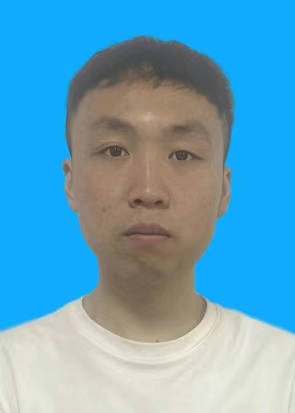
\includegraphics[width=1in,height=1.25in,clip,keepaspectratio]{./fig/slef.jpg}}]{Jiahao Xiang}
  is pursuing a Master's degree in Electronic Information at Hengyang Normal University, China. His research focuses on cryptographic engineering and efficient implementations of block ciphers on resource-constrained devices. Publications include works on lightweight cryptography optimization and contributions to open-source cryptographic projects.
\end{IEEEbiography}

\begin{IEEEbiography}[{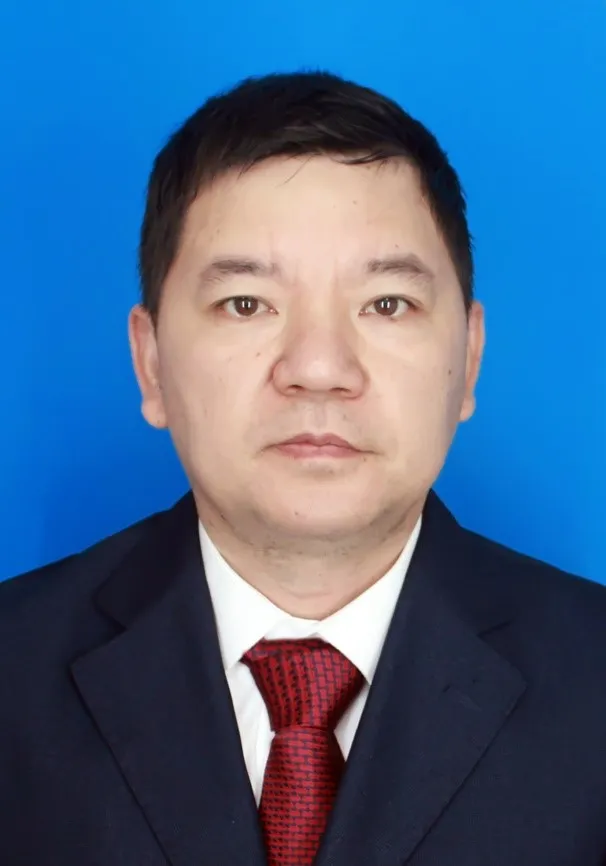
\includegraphics[width=1in,height=1.25in,clip,keepaspectratio]{./fig/boss.png}}]{Lang Li}
  received his Ph.D. and Master's degrees in computer science from Hunan University, Changsha, China, in 2010 and 2006, respectively, and earned his B.S. degree in circuits and systems from Hunan Normal University in 1996. Since 2011, he has been working as a professor in the College of Computer Science and Technology at the Hengyang Normal University, Hengyang, China. He has research interests in embedded system and information security.
\end{IEEEbiography}

% \vspace{11pt}

% \bf{If you will not include a photo:}\vspace{-33pt}
% \begin{IEEEbiographynophoto}{Jiahao Xiang}
%   is pursuing a Master's degree in Electronic Information at Hengyang Normal University, China. His research focuses on cryptographic engineering and efficient implementations of block ciphers on resource-constrained devices. Publications include works on lightweight cryptography optimization and contributions to open-source cryptographic projects.
% \end{IEEEbiographynophoto}

% \begin{IEEEbiographynophoto}{Lang Li}
%   received his Ph.D. and Master's degrees in computer science from Hunan University, Changsha, China, in 2010 and 2006, respectively, and earned his B.S. degree in circuits and systems from Hunan Normal University in 1996. Since 2011, he has been working as a professor in the College of Computer Science and Technology at the Hengyang Normal University, Hengyang, China. He has research interests in embedded system and information security.
% \end{IEEEbiographynophoto}

\end{document}